%%%%%%%%%%%%%%%%%%%%%%%%%%%%%%%%%%%%%%%%%%%%%%%%%%%%%%%%%%%%%%%%%%%%%%%%%%%%%%%%
%2345678901234567890123456789012345678901234567890123456789012345678901234567890
%        1         2         3         4         5         6         7         8

\documentclass[letterpaper, 10 pt, conference, english]{ieeeconf}  % Comment this line out if you need a4paper

\usepackage{amsmath, xparse}
\usepackage{amstext}
\usepackage{amsfonts}
\usepackage{float}
\usepackage{graphicx}
\usepackage{outlines}
% \usepackage{titling}

%\documentclass[a4paper, 10pt, conference]{ieeeconf}      % Use this line for a4 paper

% \IEEEoverridecommandlockouts                              % This command is only needed if
                                                          % you want to use the \thanks command

% \overrideIEEEmargins                                      % Needed to meet printer requirements.

%In case you encounter the following error:
%Error 1010 The PDF file may be corrupt (unable to open PDF file) OR
%Error 1000 An error occurred while parsing a contents stream. Unable to analyze the PDF file.
%This is a known problem with pdfLaTeX conversion filter. The file cannot be opened with acrobat reader
%Please use one of the alternatives below to circumvent this error by uncommenting one or the other
%\pdfobjcompresslevel=0
%\pdfminorversion=4

% See the \addtolength command later in the file to balance the column lengths
% on the last page of the document

% The following packages can be found on http:\\www.ctan.org
%\usepackage{graphics} % for pdf, bitmapped graphics files
%\usepackage{epsfig} % for postscript graphics files
%\usepackage{mathptmx} % assumes new font selection scheme installed
%\usepackage{times} % assumes new font selection scheme installed
%\usepackage{amsmath} % assumes amsmath package installed
%\usepackage{amssymb}  % assumes amsmath package installed


\title{\LARGE \bf
Project Proposal

}


\author{Arrian Chi% <-this % stops a space
\\ 
\\
% \\
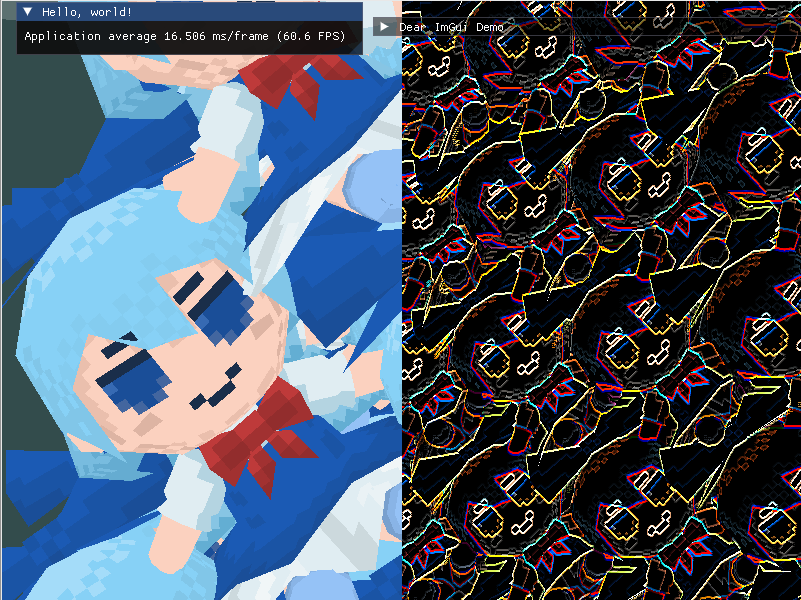
\includegraphics[width=5cm]{fumo.png} \> 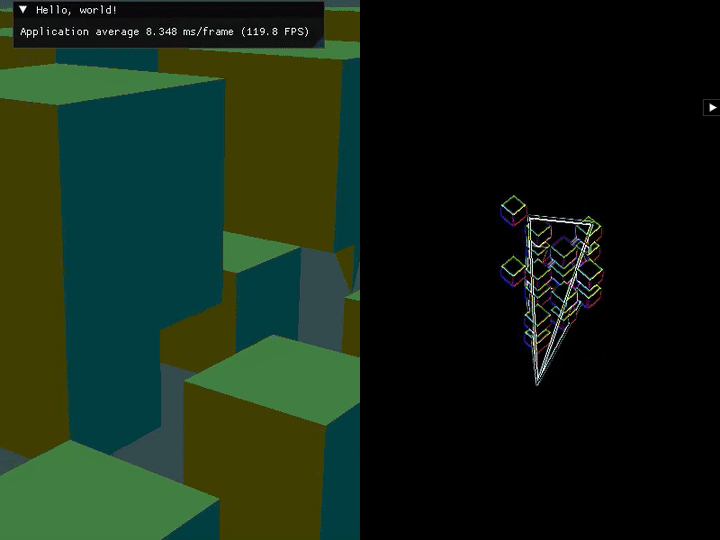
\includegraphics[width=5cm]{output.png} 
}

% \titlepic{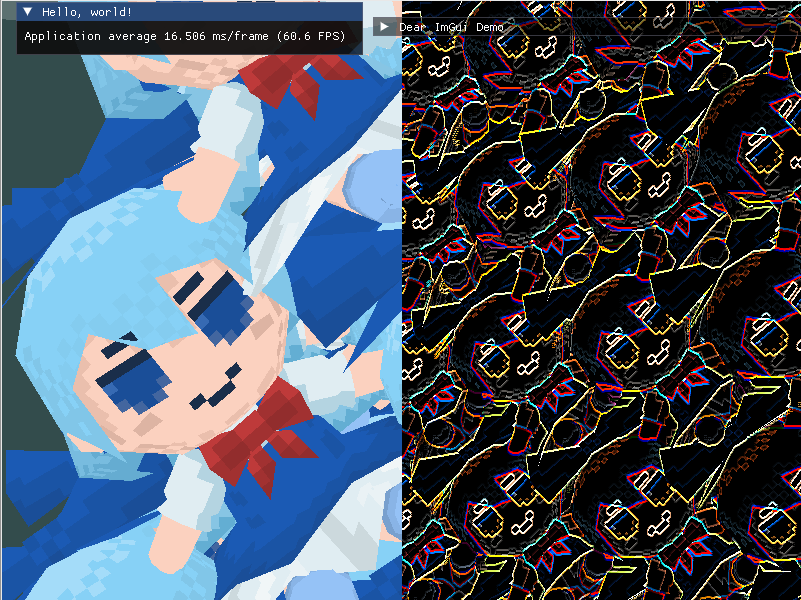
\includegraphics[width=0.45\textwidth,keepaspectratio]{fumo.png}}

\begin{document}
% \titlepic{\includegraphics[width=\textwidth]{mypicture.png}}
% \titlehead{\centering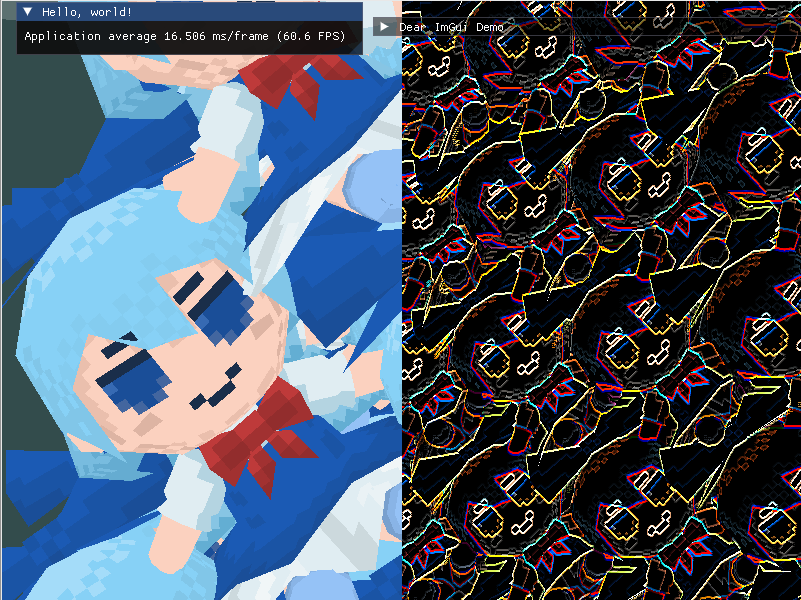
\includegraphics[width=6cm]{fumo.png}}
% \posttitle{
%         \\[\bigskipamount]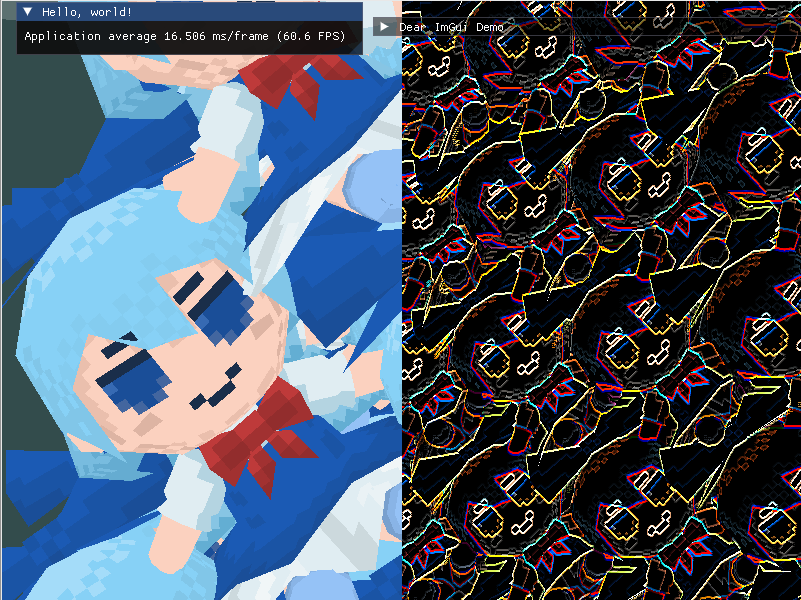
\includegraphics[width=5cm]{fumo.png}
%         \end{center}
% }


% \centering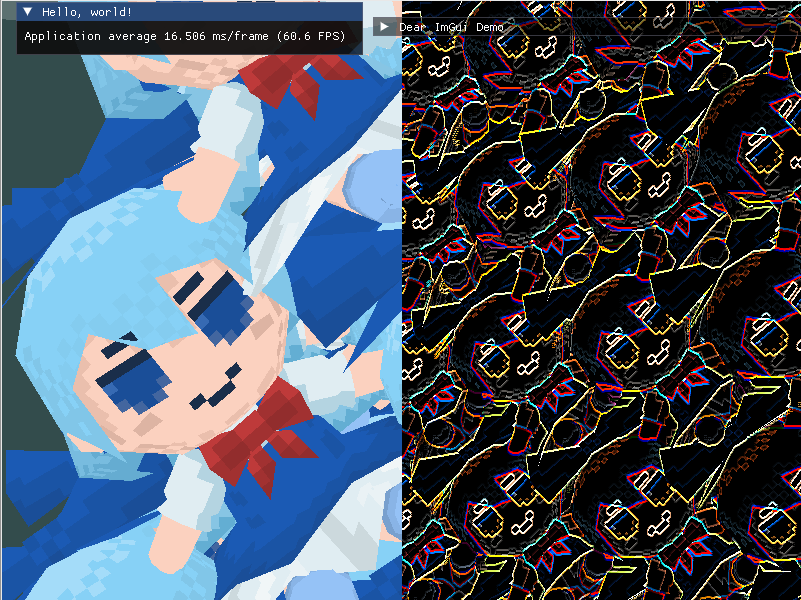
\includegraphics[width=0.45\textwidth,keepaspectratio]{fumo.png}

\maketitle


\thispagestyle{empty}
\pagestyle{empty}





%%%%%%%%%%%%%%%%%%%%%%%%%%%%%%%%%%%%%%%%%%%%%%%%%%%%%%%%%%%%%%%%%%%%%%%%%%%%%%%%

\begin{abstract}
In this proposal, I describe my interest in developing a cloth simulation feature for my hobby project, AlienGLRenderer. I will first explain the motivation of the project, followed by the questions I aim to answer, and ending with the areas I will look into for these answers. I will also provide a timeline and extra topics this project may introduce. 

\end{abstract}
\section{Introduction}
Cloth simulation is a problem with extensive research in the field of computer graphics. Numerous methods and techniques have been posed to simulate cloth. One method proposes a geometric solution, simply approximating the appearance of cloth (wrinkles, fold, etc.) based on a geometric model from cable theory \cite{weil1986synthesis}. Another proposes a physical solution involving the division of the cloth into evenly distributed masses connected by mass-spring dampers \cite{provot1995deformation}. A more well-known physically based method involves the consideration of elastic energies \cite{terzopoulos1987elastically} and forces over the surface of the cloth, which is then solved using numerical methods \cite{baraff1998large}. More recently, machine learning techniques, such as deep neural networks and unsupervised learning, have been adapted as an optimization scheme \cite{oh2018hierarchical}, including the handling of cloth dynamics \cite{bertiche2022neural}. In this project, I aim to focus on modeling cloth with the discrete elastic plates/shells (DEP/S) method as presented in class, as well as explore how to make this simulation "real-time".

\section{Motivation}
The motivation for this project starts with a hobby project AlienGLRenderer I am working on as of late. AlienGLRenderer is a renderer, written in C++ and OpenGL, designed to support the creation of simple scenes (inspired by the Quake Engine). The overall goal of this project is to streamline the rapid creation of simple scenes for artistic expression and to showcase evidence of technical knowledge. Thus, each feature added is one step towards the overarching goal. Currently the renderer supports a basic 3D rendering pipeline, model/scene loading, model instancing, frustum culling, compute shaders, and post-processing. The addition of a "real-time" cloth simulation feature would add many different features to the renderer and would be, by itself, a significant feature to showcase.



\section{Questions}
Before explaining what a cloth simulation would bring to my renderer, I would like to present the questions I am posing for this project:
        \begin{outline}
                \1 How do we simulate a cloth effectively and efficiently?
                        \2 What are some modifications we can use to make the DEP algorithm "real-time"?
                                \3 Are these modifications reasonable to implement?
                        \2 How does implicit and explicit integration differ in the context of cloth simulation?
                                \3 Could we afford a tradeoff between stability and speed? 
                                \3 How would offline rendering impact the application in general?
                \1 What technical problems/constraints arise when simulating cloth?
                        \2 Where could the DEP algorithm benefit from optimization?
                        \2 How do we render a cloth with good visual quality?
        \end{outline}



\section{Idea}
The addition of a cloth simulation feature to AlienGLRenderer would involve steps that could be divided in the following categories:
        \subsection*{Essential (High Priority) Features:}
                These include the implementation of features necessary for the setting up the simulation's computation and rendering. For instance, the concept of a simulation implies the existence of time stepping and animation, so a time-stepping algorithm (and discretization scheme) would be necessary. The DEP algorithm's computation of forces and energies implies the representation of cloth as a particle system (as also stated in \cite{baraff1998large}). The self-occlusion of cloth, as in the case of folding, requires a perspective of depth, which could be solved with a lighting / shadow model or texture mapping. Finally, depending on the speed of the DEP implementation, the application may require a offline rendering feature to precompute the cloth's state (more on this in the next section).

        \subsection*{Focus (MAIN PRIORITY) Feature:}
                The main focus of this project is to make the cloth simulation "real-time". The use of "Real-time" is in quotes because of the uncertain nature of how fast the DEP algorithm could be (when implemented in C++). For an online simulation, one iteration of the loop should take at most 33 milliseconds (30 frames per second was the common standard for games in the past). The computation time depends on a number of factors, such as the number of faces on the cloth, the size of the time step, the complexity of calculating the forces, the complexity of rendering the cloth, and more. Moreover, optimizations in the DEP algorithm are possible with GPU solvers \cite{bolz2003sparse}, better numerical methods \cite{Tamstorf2013discrete}, and neural networks \cite{bertiche2022neural}. These are areas I would like to explore to answer whether or not the DEP algorithm can be made "real-time" (online).

                However, even if it is not possible to hit the 30 FPS target, it is still possible to animate the cloth in real-time with offline-rendering (precomputing the cloth's state for set time frame). Given ample memory and time, the application would calculate all the positions for the cloth particles for every time step, store them in memory, and then render the entire animation (this is exactly how some movies ray-trace their scenes). This offline computation scheme could still benefit from optimizations; the reduction in time would cut the precompute time. That being said, although the offline rendering feature is a good fallback, I ideally want to keep my renderer online.

                \subsection*{Extra (Low Priority) Features:}
                These are features that are not necessary for the simulation to work, but would be nice to have. To name one, collision detection would make our simulation more realistic, preventing the cloth from intersecting with other objects and itself\cite{baraff1998large}. Another feature could be the simulation of wind, water, and other dynamic natural phenomena affecting the external forces of the system, which would make the simulation more lively and interesting. This could also be extended to adding destructive behaviors, such as burning and tearing, which directly impact the geometry and DOFs of the cloth. Lastly, we could add human interaction into the simulation, such as grabbing and pulling the cloth, which is essentially raycasting onto the cloth and fixing DOFs/applying forces to the selected area.
                
                It is important to note that although these features would be exciting to implement, they may contribute to not only the complexity of the project, but also the time of the computation. Take self collision detection, for example. Without the use of acceleration data structures (spatial hash maps, bounding volume hierarchies, etc.), detecting whether an edge intersects another edge is an $O(n^2)$ operation \cite{baraff1998large}. It is likely that this added feature could become a bottleneck if all of the other computation has a lower amortized time complexity. In addition, some collision detection methods could contribute to the instability of the simulation if not implemented correctly. For instance, the use of a repulsive force field around each cloth particle is reported to give subpar results\cite{Fisher}.  Thus, care must be taken before deciding to implement any of these extra features.
                
\section{Plan}
Here, I provide an overview of what the next five weeks of the project's development will look like:
        \subsection*{Week 1: Proposal}
                \begin{itemize}
                        \item Implement a simple particle system, lighting, and the DEP algorithm in C++.
                        \item Spend some time looking into various ways to optimize the algorithm.
                \end{itemize}
        \subsection*{Week 2:}
                \begin{itemize}
                        \item Determine whether the DEP algorithm can be made "real-time" (choose between offline and online rendering).
                        
                        \item Prepare the midterm report and presentation for next week.
                \end{itemize}
        \subsection*{Week 3: Midterm}
                \begin{itemize}
                        \item Present the current results and determine what is left for the project. 
                        \item If time permits, prioritize implementing interaction features before collision.
                \end{itemize}
        \subsection*{Week 4:}
                \begin{itemize}
                        \item Complete additional features in addition to polish of visual aesthetics.
                        \item Prepare the final report and presentation for next week.
                \end{itemize}
        \subsection*{Week 5:}
                \begin{itemize}
                        \item Present final results and reflect on the project.
                        \item Figure out if the project can be extended further into capstone.
                \end{itemize}


\section{Conclusion}
In this proposal, I have described my interest in developing a cloth simulation feature for my hobby project, AlienGLRenderer. I have explained what questions I hope to answer and the methods and areas I will explore first. I have also introduced the possibilty of extending this project with extra features and possibly making this my capstone. All in all, I am excited to see how this project will turn out and what it will bring to my renderer.


% \begin{figure}[!ht]
%         \centering
%         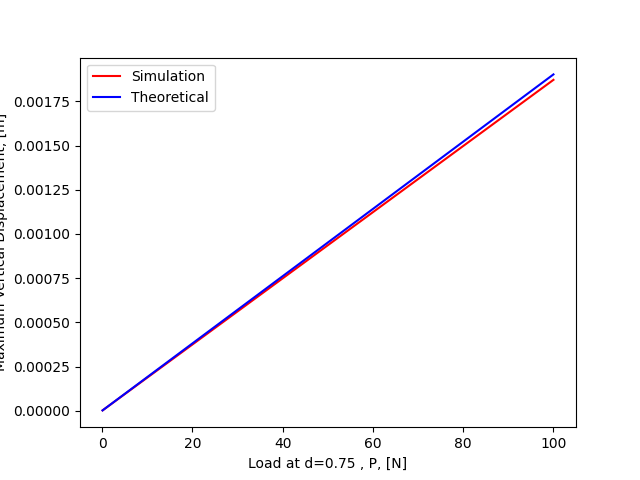
\includegraphics[width=0.45\textwidth,keepaspectratio]{p3_implicit_maxvert2xzoomed.png}
%         \caption{Plot of Maximum Vertical Displacement of the Beam v.s. the size of the point load (zoomed in again)}
%         \label{"fig:p3q2_benefit_zoomed2x"}
% \end{figure}

\addtolength{\textheight}{-12cm}   % This command serves to balance the column lengths
                                  % on the last page of the document manually. It shortens
                                  % the textheight of the last page by a suitable amount.
                                  % This command does not take effect until the next page
                                  % so it should come on the page before the last. Make
                                  % sure that you do not shorten the textheight too much.

%%%%%%%%%%%%%%%%%%%%%%%%%%%%%%%%%%%%%%%%%%%%%%%%%%%%%%%%%%%%%%%%%%%%%%%%%%%%%%%%



%%%%%%%%%%%%%%%%%%%%%%%%%%%%%%%%%%%%%%%%%%%%%%%%%%%%%%%%%%%%%%%%%%%%%%%%%%%%%%%%




\bibliographystyle{ieeetr} % We choose the "plain" reference style
\bibliography{refs} % Entries are in the refs.bib file

\end{document}
